\documentclass[aps,prl,showpacs,amsmath,twocolumn,superscriptaddress,floatfix,nofootinbib,notitlepage]{revtex4-2}

\usepackage{bm,color,xcolor,amsfonts,amsmath,amssymb,epsfig,esint,orcidlink,slashed,braket}

\usepackage[utf8]{inputenc}

\usepackage[T2A]{fontenc}
\usepackage{bbm}
\usepackage{xspace}
\usepackage{enumitem}
\usepackage{tikz}
\usepackage{lipsum}
\usetikzlibrary{calc}
\usetikzlibrary{positioning}
\usepackage[german]{varioref}
\RequirePackage[compat=1.1.0]{tikz-feynman}
\RequirePackage[compat=1.1.0]{tikz-feynhand}
\usepackage{float}
\usepackage{commath}
\usepackage{booktabs}
\usepackage[normalem]{ulem}

\allowdisplaybreaks

\newcommand{\subsubsubsection}[1]{\paragraph{#1} ~ \vspace{1.7ex plus 0.2ex}}

\newenvironment{todo}%
{\large \textsc{Todo:} \normalsize \begin{itemize} \color{blue}}%
{\end{itemize}}

\newcommand{\red}[1]{{\color{red}#1}}
\newcommand{\blue}[1]{{\color{blue}#1}}
\DeclareRobustCommand{\magenta}[1]{{\color{magenta}#1}}
\newcommand{\fkcomment}[1]{{\color{blue}[FK: #1]}}
\newcommand{\chhcomment}[1]{{\color{red}[CH: #1]}}
\newcommand{\ancomment}[1]{{\color{blue}[AN: #1]}}
\newcommand{\fk}[1]{{\color{blue}#1}}
\newcommand{\ch}[1]{{\color{green}#1}}
\newcommand{\an}[1]{{\color{blue}#1}}
\newcommand{\pp}[1]{{\color{orange}[PP: #1]}}

\newcommand{\bbnP}{[\bar{b}b]_1(nP)}
\newcommand{\bbarb}{[\bar{b}b]_1}
\newcommand{\tauEB}{\hat{\cal J}}
\newcommand{\tauinv}{\hat\tau^{-1}}
\newcommand{\dtauinvEB}{\Bigl[\partial_E\hat\tau^{-1}\Bigr]_{E=-E_B}}
\newcommand{\psibb}{\Psi^{(\bar{b}b)}}
\newcommand{\Mbb}{M^{(\bar{b}b)}}

\setcounter{secnumdepth}{3}

\newcommand{\GeV}{\mathrm{GeV}}
\newcommand{\MeV}{\mathrm{MeV}}
\newcommand{\vep}{{\bm p}}
\newcommand{\vek}{{\bm k}}
\newcommand{\veq}{{\bm q}}
\newcommand{\ver}{{\bm r}}
\newcommand{\vex}{{\bm x}}
\newcommand{\veA}{{\bm A}}
\newcommand{\vetau}{{\bm \tau}}
\definecolor{green}{RGB}{44,160,44}
\definecolor{omeRevision}{RGB}{0,105,105}
\newcommand{\be}{\begin{equation}}
\newcommand{\ee}{\end{equation}}
\newcommand{\bea}{\begin{eqnarray}}
\newcommand{\eea}{\end{eqnarray}}
\newcommand{\beas}{\begin{eqnarray*}}
\newcommand{\eeas}{\end{eqnarray*}}
\newcommand{\ds}{\displaystyle}
\newcommand{\B}{\color{blue}}
\newcommand{\R}{\color{red}}
\newcommand{\G}{\color{green}}
\newcommand{\veL}{{\bm L}}
\newcommand{\veS}{{\bm S}}
\newcommand{\ven}{{\bm n}}

\newcommand{\nn}{\notag}
\newcommand{\dk}{\frac{d^3k}{(2\pi)^3}}
\newcommand{\ddq}{\frac{d^3q}{(2\pi)^3}}
\newcommand{\ddqpr}{\frac{d^3q'}{(2\pi)^3}}
\newcommand{\dqr}{\frac{q^2dq}{2\pi^2}}
\newcommand{\dqrpr}{\frac{q^{\prime2}dq'}{2\pi^2}}
\newcommand{\ddp}{\frac{d^3p}{(2\pi)^3}}
\newcommand{\ddpp}{\frac{d^3p'}{(2\pi)^3}}
\newcommand{\intp}{\int\frac{d^3p}{(2\pi)^3}}
\newcommand{\intk}{\int\frac{q^2dq}{(2\pi)^3}}
\newcommand{\bb}{\bar{b}b}
\newcommand{\qq}{q\bar{q}}
\newcommand{\QQ}{\bar{b}b}
\newcommand{\gpi}{g_b}
\renewcommand{\vec}{\bm}
\newcommand{\no}{\notag\\}
\newcommand{\Hoo}{H_{\rm MM}}
\newcommand{\Hot}{V_{ls}}
\newcommand{\Htt}{V_{s}}
\newcommand{\mG}{m_\phi}
\newcommand{\EG}{E_\phi}
\newcommand{\CSOME}{C_S^{\rm (OME)}}
\newcommand{\COOME}{C_O^{\rm (OME)}}
\newcommand{\CSQM}{C_S^{(\QQ)}}
\newcommand{\COQM}{C_O^{(\QQ)}}
\newcommand{\CSOQM}{C_{SO}^{(\QQ)}}
\newcommand{\En}{E_n}
\newcommand{\Enzero}{E_n^{(0)}}
\newcommand{\Eizero}{E_i^{(0)}}
\newcommand{\VR}{V_R}
\newcommand{\gc}{g_c}
\newcommand{\X}{X(3872)}
\newcommand{\Xb}{X_b}
\newcommand{\gev}{GeV}
\newcommand{\mev}{MeV}
\newcommand{\Yb}{\Upsilon(10753)}
\newcommand{\Yfour}{\Upsilon(10580)}
\newcommand{\Yfive}{\Upsilon(10860)}
\newcommand{\Ysix}{\Upsilon(11020)}
\newcommand{\Dszero}{D^*_{s0}(2317)}
\newcommand{\veep}{{\bm \epsilon}}
\newcommand{\veepst}{{\bm \epsilon}^{\prime*}}
\newcommand{\tbd}[1]{{\color{red}[TODO: #1]}}
\newcommand{\unit}[1]{~(#1)}
\newcommand{\BOchiEFT}{BO$\chi$EFT\xspace}

\newcommand{\VQQ}{V^{(\bar{b}b)}}
\newcommand{\VOME}{V^{\rm (OME)}}
\newcommand{\calH}{{\cal H}}
\newcommand{\hatH}{H}
\newcommand{\tilH}{\tilde{{\cal H}}}


\newcommand{\rub}{\affiliation{Institut f\"ur Theoretische Physik II, Ruhr-Universit\"at Bochum, D-44780 Bochum, Germany }}

\newcommand{\bonn}{\affiliation{Helmholtz-Institut f\"ur Strahlen- und Kernphysik and Bethe Center for Theoretical Physics,\\ Universit\"at Bonn, D-53115 Bonn, Germany}}

\newcommand{\fzj}{\affiliation{Institute for Advanced Simulation
and Cluster of Excellence ``Color meets Flavor'', Forschungszentrum J\"ulich, D-52425 J\"ulich, Germany}}

\newcommand{\itp}{\affiliation{Institute of Theoretical Physics, Chinese Academy of Sciences, Beijing 100190, China}}

\newcommand{\ucas}{\affiliation{School of Physical Sciences, University of Chinese Academy of Sciences, Beijing 100049, China}}

\newcommand{\lis}{\affiliation{CeFEMA, Center of Physics and Engineering of Advanced Materials, Instituto Superior T{\'e}cnico, Avenida Rovisco Pais 1, 1049-001 Lisboa, Portugal}}

\newcommand{\tum}{\affiliation{
Technical University of Munich, TUM School of Natural Sciences, Physics Department, 85748 Garching, Germany}}

\newcommand{\scnt}{\affiliation{Southern Center for Nuclear-Science Theory (SCNT), Institute of Modern Physics,\\ Chinese Academy of Sciences, Huizhou 516000, China}}

\newcommand{\hiskp}{\affiliation{Helmholtz-Institut f\"ur Strahlen- und Kernphysik, Universit\"at Bonn, 53115 Bonn, Germany}}

\newcommand{\hohai}{\affiliation{College of Mechanics and Engineering Science, Hohai University, Nanjing 211100, China}}


\graphicspath{{Figs.dir/}}

\begin{document}

\title{Towards Born-Oppenheimer chiral effective field theory}

\author{Yu Zhang\orcidlink{0009-0007-2951-6536}}\email{zhangyu@itp.ac.cn}
\itp\ucas

\author{Feng-Kun~Guo\orcidlink{0000-0002-2919-2064}}
\email{fkguo@itp.ac.cn}
\itp\ucas\scnt

\author{Christoph~Hanhart\orcidlink{0000-0002-3509-2473}}\email{c.hanhart@fz-juelich.de}
\fzj

\author{Alexey Nefediev\orcidlink{0000-0002-9988-9430}}\email{nefediev@hiskp.uni-bonn.de}
\hiskp

\author{Paul P\"utz\orcidlink{0009-0007-0783-6520}}\email{paul.puetz@tum.de}
\tum

\begin{abstract}
We introduce Born--Oppenheimer chiral effective field theory (\BOchiEFT), a novel framework
for comprehensive studies of generic and exotic hadron spectroscopy, that combines systematically quark and hadronic degrees of freedom with meson-exchange interactions provided by chiral effective field theory. We set up the leading order and discuss the power counting of all relevant interactions.
As a first proof-of-concept application, we employ \BOchiEFT to study the bottomonium sector with $J^{PC}=1^{++}$ and discuss various scenarios for the $\Xb$, the heavy-flavour counterpart of the $\X$.
\end{abstract}

\maketitle


{\it Introduction.}---The discovery of the enigmatic state $\X$ by the Belle Collaboration in 2003~\cite{Belle:2003nnu} initiated a systematic study of exotic hadrons\u2014states that defy the conventional structure of mesons and baryons as $q\bar q$ and $qqq$, respectively (for recent reviews, see Refs.~\cite{Ali:2017jda,Guo:2017jvc,Olsen:2017bmm,Albuquerque:2018jkn,Liu:2019zoy,Guo:2019twa,Brambilla:2019esw,Chen:2022asf,Liu:2024uxn,Chen:2024eaq,Wang:2025sic,Dai:2026fkg,Bai:2026atm}). Since it contains $c\bar{c}$ and has the quantum numbers $J^{PC}=1^{++}$, it is designated by the Particle Data Group (PDG) as $\chi_{c1}(3872)$. Although 
more than 20 years have passed since the discovery of the $\X$, 
its nature and properties are still under active debate. During this time, the family of exotic states in both the charm and bottom sectors has been enriched by several dozen new members, calling for a unified framework to describe them.

Nowadays, our knowledge about quantum chromodynamics (QCD) in the nonperturbative regime relies on two key pillars: high-energy experimental data and first-principle lattice calculations. The latter provide unique access to quantities unattainable experimentally, such as static $Q\bar Q$ potentials. However, synthesising these two fundamental sources of insight into a coherent theoretical picture is challenging because of the disparate degrees of freedom operating at different distance scales: quarks and gluons at short distances versus hadrons at long distances, exceeding $1/\Lambda_{\rm QCD}$. 
To bridge this gap, we propose a novel theoretical framework dubbed Born--Oppenheimer (BO) chiral effective field theory (\BOchiEFT) that, upon construction, will seamlessly combine hadronic effective field theories with the scale separation under the BO approximation~\cite{Born:1927} for slow heavy quarks and fast light quarks and gluons, also exploited in the BOEFT developed in Refs.~\cite{Braaten:2014qka,Berwein:2015vca,Brambilla:2017uyf,Oncala:2017hop,Soto:2020xpm,Berwein:2024ztx,Brambilla:2026jqz}.
The powerful strength of the \BOchiEFT is that
it combines
the well developed chiral EFT, thus
rigorously accounting for long-range light-meson exchanges and hadronic molecular dynamics~\cite{Baru:2010ww,Hanhart:2011jz,Guo:2016bjq,Hammer:2016prh,Hanhart:2022qxq}, with the BO framework, which naturally incorporates static heavy-quark potentials directly extracted in lattice-QCD studies. This promising connection did not exist up to now. 

As a proof-of-concept application, we employ LO \BOchiEFT to investigate the $J^{PC}=1^{++}$ bottomonium spectrum. By solving the Lippmann--Schwinger equation (LSE) for the $B\bar{B}^*$-$B^*\bar{B}^*$ coupled-channel scattering amplitudes and extracting the poles in the complex energy plane, we perform a comprehensive study of the excited $\chi_{b1}(nP)$ ($n=1,2,3$) states and the elusive $X_b$ as the heavy-flavour analogue of the $\X$.
We conclude that the state with a mass about 10.513~GeV, which has been long regarded as the $\chi_{c1}(3P)$, could well be the $X_b$.

{\it Interaction potential at LO.}---At LO of \BOchiEFT, the $B\bar{B}^*$ interaction potential comprises $\VOME$ for the one-meson exchange (OME) of ground-state pseudoscalar $\pi$ and $\eta$ mesons, $\VQQ$ for an $s$-channel interaction mediated by
a sum of quark--antiquark states truncated at some $N$, and a short-range contact term $C$ that depends on $N$ as well as $\Lambda$, a regulator introduced to render the scattering equation introduced in Eq.~\eqref{LSEfull2} well defined,
\be
V=\VOME+\sum_{n=1}^N \VQQ_n+C(\Lambda,N).
\label{Vdef}
\ee
The masses and wave functions that enter $\VQQ$ come from a Schr{\"o}dinger equation,
\be
\left[2m_b-\frac{1}{m_b}\nabla^{2}+V(r)\right]\psibb=\Mbb\psibb,
\label{Scheq}
\ee
with the LO static, spin-independent, colour-singlet Cornell potential,
\be
V(r)=
V_0+
\sigma r+\frac{\gamma}{r},\quad \gamma\equiv-\frac43\alpha_s<0.
\label{Cornell}
\ee
This setup aligns with the lattice-QCD study of Ref.~\cite{Bulava:2024jpj}, which extracts the physical parameters to be
\be
\sigma=0.198~\mbox{GeV}^2,\quad
\gamma=-0.434.
\label{eq:parameters}
\ee
The role of the parameter $V_0$ is discussed below. Static-limit lattice calculations cannot determine the $b$-quark mass, so we adopt
\be
m_b=4.534~\mbox{GeV},
\label{mb}
\ee
which complies well with typical values employed in quark models. This choice will be further motivated below.
For the $\bbnP$ states,
which denote the $\bar bb$ states with $1^{++}$
quantum numbers, the wave functions read
\be
\psibb_{n,L=1}(r)=Y_{1m}(\hat{\ver})R_{1n}(r),
\label{psi}
\ee
with $Y_{1m}(\hat{\ver})$ and $R_{1n}(r)$ being the $L=1$ spherical harmonics and the radial wave function, respectively.

At LO in the adopted power counting, quarkonium states couple directly only to the $S$-wave $B\bar{B}^*(^3S_1)$ channel, so the wave function of a physical state reads
\be
|\Psi\rangle=
\begin{pmatrix}
\lambda_1\ket{\bbarb(1P)}\\ \lambda_2\ket{\bbarb(2P)}\\ \cdots\\ \phi(q)\ket{B\bar{B}^*}
\end{pmatrix},\quad \braket{\Psi|\Psi}=1,
\label{state}
\ee
with the probability of finding compact bottomonium components in the bound state wave function given by
\be
{\cal P}_{\bar{b}b}
=\sum_{n=1}^N|\lambda_n|^2,
\label{Pbb}
\ee
and the $S$-wave-projected 
short-range
potential is \cite{Zhang:2026iyr}
\be
V^{(\QQ)+{\rm CT}}_S(p',p)=\frac{g^2}{4\pi}
\sum_{n=1}^N\frac{\psi_n(p')\psi^*_n(p)}{M-\Mbb_n}+C(N),
\label{VQMab}
\ee
where $\Mbb_n$ incorporates the parameter $V_0$ from Eq.~\eqref{Cornell}. Hereafter, energies $E=M-M_{\rm th}$ and $\En=\Mbb_n-M_{\rm th}$ are measured relative to the open-bottom $B\bar{B}^*$ threshold,
\be
M_{\rm th}=m_B+m_{B^*}.
\label{Mth}
\ee
The $n$-independent coupling constant $g$ is defined via the matrix element of the transition operator $\hat{g}$ between the $n$-th bottomonium state and $B\bar{B}^*(^3S_1)$,
\be
\braket{B\bar{B}^*(^3S_1)|\hat{g}|\bbnP}=g\psi_n(p).
\label{psigMM}
\ee
The form factor $\psi_n$ is linked to the radial wave function,
\be
\psi_n(p)=
4\pi \int_0^\infty r^2dr\, j_0(pr)R_{1n}(r),
\label{psinp}
\ee
where $j_0(z)$ is the zeroth-order spherical Bessel function \cite{Zhang:2026iyr}. We detail the determination of $g$ below.

Crucially, while LO quarkonium states couple exclusively to the $S$-wave $B\bar{B}^*(^3S_1)$ channel, the OME interaction dynamically couples all relevant $S$- and $D$-wave open-bottom channels with $J^{PC}=1^{++}$,
\be
\{B\bar{B}^*(^3S_1),B\bar{B}^*(^3D_1),B^*\bar{B}^*(^5D_1)\},
\label{BBchannels}
\ee
labeled by $\alpha=1,2,3$, respectively.
In time-ordered perturbation theory (TOPT), OME within the $B^{(*)}\bar{B}^*$ system involves four 3-body intermediate states,
\be
\{B\bar{B}\phi,B^*\bar{B}^*\phi,B\bar{B}^*\phi,\bar{B}^*B\phi\},
\label{BBphichannels}
\ee
where $\phi$ represents the exchanged $\pi$ or $\eta$ meson.
The corresponding OME potentials are given explicitly in the End Matter (see also the companion paper~\cite{Zhang:2026iyr}).
Note that there are two components in the $C$-even $B\bar{B}^*$ state:
\be
\left|B \bar{B}^* ; C=+\right\rangle=\frac{1}{\sqrt{2}}\left(\left|B \bar{B}^*\right\rangle-\left|B^* \bar{B}\right\rangle\right).
\ee


{\it Power counting and higher orders.}---Let $Q$ denote a generic momentum scale below the EFT hard scale $\Lambda$, also taken to be the momentum cutoff introduced to regularise the LSE.
In the \BOchiEFT power counting, each $S$-wave $[\bar{b}b]_1B\bar{B}^*$ vertex in the $s$-channel $\bbnP$ exchange scales as $\mathcal{O}(Q^0)$. For states lying close to the $B\bar{B}^*$ threshold [energy separation $\sim \mathcal{O}(Q^2/(2\mu))$, with $\mu$ the reduced $B\bar{B}^*$ mass], the exchange propagator is kinematically enhanced to $\mathcal{O}(Q^{-2})$. Such states must be explicitly retained in the sum in Eq.~\eqref{Vdef}, necessitating a sufficiently large $N$. Conversely, for states well separated from the threshold, both the propagator and exchange contribution scale as $\mathcal{O}(Q^0)$. Being analytic for momenta $\sim Q$, the contribution of these radially excited states does not induce strong energy dependence and can be absorbed into the $\mathcal{O}(Q^0)$ local counterterm $C(N)$.

By parity conservation, $B^{(*)}$ mesons emit light pseudoscalar mesons in $P$ wave, thus assigning $\mathcal{O}(Q)$ scaling to each chiral vertex. Two vertices combined with the $\mathcal{O}(Q^{-2})$ light-meson propagator result in $\VOME$ potential scaling $\mathcal{O}(Q^0)$. Because the $\pi$- and $\eta$-exchange potentials possess left-hand cuts with the branch points inside the studied energy range, their effects cannot be Taylor-expanded into derivative-based local operators and must be explicitly retained in $\VOME$. To ensure  renormalisability, this OME interaction must be accompanied by a short-range contact interaction $C(\Lambda)$~\cite{Baru:2015nea}. Crucially, this contact term also encapsulates the dynamics of heavier, integrated-out channels like $B_s^{(*)}\bar{B}^{(*)}_s$.

Consequently, the short-range parameter $C$ depends essentially on both the hard cutoff $\Lambda$ and the truncation integer $N$, as reflected in Eq.~\eqref{Vdef}. For a properly formulated theory, physical observables are insensitive to the cutoff $\Lambda$ and $N$. In the calculations below, we set $N=4$ and $\Lambda=4$~GeV and verified that variations in both $\Lambda$ and $N$ can be compensated by adjusting $C$.

Proceeding to higher orders of \BOchiEFT implies that momentum-dependent counterterms and multi-meson exchanges should be incorporated, while the quark--antiquark states and their wave functions should be calculated using an interquark potential of higher order in potential nonrelativistic QCD~\cite{Brambilla:1999xf,Brambilla:2000gk,Pineda:2000sz,Brambilla:2004jw}. Momentum-dependent counterterms can also generate short-distance contributions to higher partial waves as well as transitions between different partial waves. These two extensions are controlled by distinct expansion parameters: the ratio of the inter-meson momentum and pion mass to the typical hadronic scale, and the ratio of the typical momentum to the heavy-quark mass, respectively. The interplay between these two expansions and the estimation of the associated theoretical uncertainties will be investigated in future work.

{\it BO degrees of freedom in \BOchiEFT.}---A systematic separation of slow heavy-quark dynamics from fast light-quark and gluon dynamics can be achieved using the BO approach~\cite{Born:1927}, which has a long history in hadronic physics. Its earliest applications to multiquark systems date to almost half a century ago~\cite{Chao:1979tg}. Later, heavy hybrid quarkonia were extensively studied within this framework~\cite{Griffiths:1983ah,Juge:1997nc,Juge:1997nd,Juge:1999ie,Guo:2008yz,Soto:2017one,Brambilla:2018pyn,Brambilla:2019jfi}, which was then extended to heavy exotic $XYZ$ mesons~\cite{Braaten:2014qka} and formulated as an EFT, the BOEFT~\cite{Brambilla:2017uyf}.

One crucial part of the BO approximation is that at leading order, the $b$ and $\bar{b}$ sources are static and thus define a spatial axis $\hat{\ver}$, giving rise to (i) cylindrical, (ii) $PC$, and (iii) reflection symmetries with respect to a plane containing this axis. The corresponding irreducible representations (irreps) are tagged as $\Lambda_\eta^\sigma$, where
\begin{itemize}
\item $\Lambda=|\lambda_\ell|$ is the modulus of the projection of $\bm{j}_\ell$ (the total momentum of the light degrees of freedom) onto the axis $\hat{\ver}$, with $\Lambda=0,1,\dots$ conventionally denoted as $\Sigma,\Pi,\dots$, respectively;
\item $\eta=g,u$ denotes even or odd $PC$, respectively, of the light degrees of freedom;
\item $\sigma=P(-1)^{j_\ell}$ is specified only for $\Lambda=0$.
\end{itemize}

In the heavy-quark limit $m_b{\to}\infty$, the eigenenergies of the light degrees of freedom at each fixed $b\bar{b}$ separation $r$ define the $r$-dependent, energy-independent BO potentials~\cite{Juge:1997nc,Braaten:2014qka}. In particular, for $j_{\ell}^{PC}=0^{++}$, the interaction potential in the heavy quark--antiquark pair, $\Sigma_g^+$, corresponds to the Wilson line connecting $b$ and $\bar{b}$. Coupling $\bar{b}b$ states to two-meson channels introduces additional possibilities.
To classify the multiplet structure set by heavy quark spin symmetry (HQSS) for $S$-wave interactions between hadron pairs, we note that both $j_{\ell}^{PC}$ and $s_{\bar{b}b}^{PC}$ (the $b\bar{b}$ total spin and $PC$) in the final state can be $0^{-+}$ or $1^{--}$. Then, for $j_{\ell}=0$ and 1, we have~\cite{Bondar:2011ev,Guo:2017jvc}
\be
\begin{split}
0_{\ell}^{-+} \otimes 0_{\bar{b}b}^{-+}&=0^{++},\\
0_{\ell}^{-+} \otimes 1_{\bar{b}b}^{--}&=1^{+-},\\
1_{\ell}^{--} \otimes\, 0_{\bar{b}b}^{-+}&=1^{+-},\\
1_{\ell}^{--} \otimes 1_{\bar{b}b}^{--}&=0^{++} \oplus 1^{++} \oplus 2^{++},
\label{eq:qn}
\end{split}
\ee
with $J^{PC}=1^{++}$ contained in the last relation, so the configuration $\Sigma_u^-$ with $j_\ell^{PC}=0^{-+}$ does not contribute~\cite{Berwein:2024ztx,Brambilla:2026zfw}. The longitudinal component of $1_\ell^{--}$ with $\lambda_\ell=0$ corresponds to $\Sigma_g^{+\prime}$ and its transverse components with $\lambda_\ell=\pm1$ form $\Pi_g$. These addition energy levels account for the coupling of $\bbnP$ to the $S$-wave $B\bar{B}^*$ system and for interactions between the mesons~\cite{Berwein:2024ztx,Brambilla:2026zfw}.

Inclusion of $D$-wave meson pairs in Eq.~\eqref{BBchannels} makes the situation more intricate. There are two ways to couple the heavy spin $s_{\bar{b}b}=1$, the angular momentum of the light degrees of freedom ${j}_\ell=1$, and the orbital angular momentum $L=0,2$ of the $B^{(*)}\bar{B}^*$ pair. Coupling $\bm{s}_{\bar{b}b}$ with $\bm{j}_\ell$ gives $S=1$ for the $C$-even $B\bar{B}^*$ pair and $S=2$ for $B^*\bar{B}^*$ ($S=0$ cannot contribute to the $1^{++}$ sector). Combining these spin states with $L$ yields the three partial-wave channels in Eq.~\eqref{BBchannels}. Alternatively, $\bm{j}_\ell$ can couple with the orbital angular momentum to $\bm{J}_\ell\equiv\bm{L}+\bm{j}_\ell$, which is conserved in the heavy-quark limit. For $L=0$ and 2, $J_\ell =1$ and 1, 2, 3, respectively. The $J_\ell=3$ component cannot couple with $s_{\bar{b}b} = 1$ to form $J^{PC}=1^{++}$. The state $|J_\ell=2,\lambda_\ell=0\rangle$ is eliminated
as the Clebsch--Gordan coefficient $\braket{L,0,1,\lambda_\ell=0|J_\ell,\lambda_\ell=0}$ vanishes for $J_\ell=L=2$. So three $J^{PC}=1^{++}$ BO configurations remain~\cite{Brambilla:2026zfw}: $\ket{\Sigma_g^{+\prime}}$ and $\ket{\Pi_g;1}$, for $J_\ell=1$,  and $\ket{\Pi_g;2}$, for $J_\ell=2$. The orthogonal transformation relating them to the partial-wave channels in Eq.~\eqref{BBchannels} is~\cite{Zhang:2026iyr},
$$
\begin{pmatrix}\ket{\Sigma_g^{+\prime}}\\[0.5mm] \ket{\Pi_g;1}\\[0.5mm] \ket{\Pi_g;2}\end{pmatrix}
=\begin{pmatrix}
\frac{1}{\sqrt3} & \frac{1}{\sqrt6} & -\frac{1}{\sqrt2}\\[1mm]
\sqrt{\frac23} & -\frac{1}{2\sqrt3} & \frac12\\[1mm]
0 & \frac{\sqrt3}{2} & \frac12
\end{pmatrix}
\begin{pmatrix}\ket{B\bar{B}^*(^3S_1)}\\[0.5mm] \ket{B\bar{B}^*(^3D_1)}\\[0.5mm] \ket{B^*\bar{B}^*(^5D_1)}\end{pmatrix}.
$$

For fixed $\bar{b}b$ sources, $\ket{\Pi_g;1}$ and $\ket{\Pi_g;2}$ share the same static potential $V_{\Pi_g}(r)$. Thus, in the basis of Eq.~\eqref{BBchannels}, the $r$-space potential for static $B^{(*)}\bar{B}^*$ channels reads
\be
V(r)
=
V_C(r)\,\mathbbm{1}
+
V_T(r)
\begin{pmatrix}
0 & -\sqrt2 & \sqrt6\\
-\sqrt2 & 1 & \sqrt3\\
\sqrt6 & \sqrt3 & -1
\end{pmatrix},
\label{eq:cylindricalstuff}
\ee
where the central and tensor radial potentials are
\be
\begin{split}
V_C(r) &= \frac13 \left[V_{\Sigma_g^{+\prime}}(r)+2V_{\Pi_g}(r)\right], \\
V_T(r) &= \frac16\left[V_{\Pi_g}(r) - V_{\Sigma_g^{+\prime}}(r) \right].
\end{split}
\label{eq:VCT-BO}
\ee

In the local static limit, the $\Sigma_g^{+\prime}$ and $\Pi_g$ potentials become degenerate as $r\to 0$ and approach the same meson-pair threshold at large distances~\cite{Berwein:2024ztx}, although they may differ substantially at intermediate distances. In \BOchiEFT, the long-range interaction is described by the potential $\VOME$ that contributes to the potential in Eq.~\eqref{eq:VCT-BO} in this limit. Meanwhile, crucially, in BO$\chi$EFT with physical bottom-meson masses, hyperfine splitting, recoil effects, and energy dependence are retained in the OME interaction (see the explicit expressions in the End Matter). Consequently, the resulting potentials at larger distances are nonlocal and do not reduce to the simple local form in Eq.~\eqref{eq:cylindricalstuff}.
Their short-range parts are parameterised through a derivative expansion of local operators in the two-hadron interaction terms. This is necessary because the two-hadron states are treated explicitly as low-energy dynamical degrees of freedom, without resolving their internal structure at short distances.
At LO in \BOchiEFT, the short-range hadron--hadron potential in the $1^{++}$ channel is therefore parameterised by the constant contact term $C$, as detailed in Eq.~\eqref{Vdef}. Higher orders include further contact terms with additional powers of the incoming and outgoing momenta $p$ and $p'$, each counted at $\mathcal{O}(Q)$~\cite{Zhang:2026iyr}. In coordinate space, these terms correspond to potentials $\propto\delta^{(3)}(\ver)$ and their derivatives. 
The nonderivative LO contact term $C$ thus contributes only to $V_{11}(p',p)$ [see Eq.~\eqref{Vcoupled} below], with $L_1=0$, where $\alpha=1$ denotes the $B\bar{B}^*(^3S_1)$ channel in Eq.~\eqref{BBchannels}. At higher orders, two- and four-derivative contact terms encode additional short-range information in the $S$--$S$, $S$--$D$, and $D$--$D$ channels. This illustrates how short-range BO potentials are encoded in the derivative expansion of \BOchiEFT and how the BO cylindrical symmetry for two static sources is incorporated into this EFT~\cite{Zhang:2026iyr}.

{\it Lattice input.}---The leading input for the interquark potential and the quarkonium couplings to open-flavour channels can be obtained from unquenched lattice studies of a static quark--antiquark pair, corresponding to the heavy-quark limit, $m_Q\to\infty$~\cite{Bulava:2019iut,Bulava:2024jpj}. In particular, Ref.~\cite{Bulava:2024jpj} investigates the static potential between bottom quark and antiquark, including string-breaking effects induced by light-quark pairs, and extracts the coupling $\sqrt{2}g_l$, with
\be
g_l=35.0(5)_{\rm stat}(3)_{\rm sys}
~\mbox{MeV},
\label{gl}
\ee
that governs the transitions between quark--antiquark states and an open-bottom channel. The two-meson operator constructed in Ref.~\cite{Bali:2005fu} and employed in Refs.~\cite{Bulava:2019iut,Bulava:2024jpj} corresponds to a pair of pseudoscalar heavy mesons $B\bar{B}$. Writing the spin wave function of each meson as $(|{\uparrow_b\downarrow_\ell}\rangle-|{\downarrow_b\uparrow_\ell}\rangle)/\sqrt2$ (where $b$ and $\ell$ denote the $b$ quark and the light degrees of freedom, respectively) and projecting onto the bases $\ket{j_\ell, \lambda_\ell}$ and $\ket{s_{\bar{b}b},m_{\bar{b}b}}$, we obtain
\be
\begin{split}
\ket{B\bar{B}}={}&\frac12\ket{0_\ell,0}\ket{0_{\bar{b}b},0}\\
&+\frac12\sum_{\lambda_\ell=\pm1,0}(-1)^{\lambda_\ell+1}
\ket{1_\ell,\lambda_\ell}\ket{1_{\bar{b}b},-\lambda_\ell}.
\label{eq:BBdecomp}
\end{split}
\ee

The static $\bar{b}b$ potential is extracted from lattice calculations~\cite{Bulava:2019iut, Bulava:2024jpj} using an interpolating operator corresponding to the symmetric spin state $\ket{1_{\bar{b}b},0}$. Selecting the corresponding term in Eq.~\eqref{eq:BBdecomp}, we find that the coupling of $\ket{1_\ell,0}\ket{1_{\bar{b}b},0}$ to $J^{PC}=1^{++}$ bottomonium acquires an additional factor of 2; see the companion paper~\cite{Zhang:2026iyr} for a detailed discussion. Note also that the total strength of the transition in Eq.~\eqref{psigMM} from $\bbnP$ to the $B^{(*)}\bar{B}^*$ states is distributed among the partial waves listed in Eq.~\eqref{BBchannels} with the coefficients $(1/\sqrt{3},1/\sqrt{6},-1/\sqrt{2})$, respectively~\cite{Baru:2016iwj,Bruschini:2023zkb}. Combining all factors, the coupling of a $J^{PC}=1^{++}$ bottomonium to an $S$-wave $B\bar{B}^*$ pair is
\be
g=2\times\frac{1}{\sqrt{3}}\times\sqrt{2}\, g_l= 57~\mbox{MeV},
\label{g}
\ee
where the central value in Eq.~\eqref{gl} was used.

{\it Application of \BOchiEFT to $\Xb$.}---In the basis of states defined in Eq.~\eqref{BBchannels}, the partial-wave projected LO potential in the $1^{++}$ sector is
\be
V_{\alpha'\alpha}(p',p)=\delta_{\alpha' 1}\delta_{\alpha 1}
V_S^{(\QQ)+{\rm CT}}(p',p)+\VOME_{\alpha'\alpha}(p',p).
\label{Vcoupled}
\ee
The $T$-matrix satisfies the partial-wave projected LSE,
\begin{align}
&T_{\alpha'\alpha}(p',p)=V_{\alpha'\alpha}(p',p) \label{LSEfull2}\\
&\quad -\sum_{\alpha''}\int_0^\Lambda\frac{q^2dq}{2\pi^2}
V_{\alpha'\alpha''}(p',q)G_{\alpha''}(k,q) T_{\alpha''\alpha}(q,p),\notag
\end{align}
where the nonrelativistic two-body Green's functions are
\be
\begin{split}
&G_1(k,q)=G_2(k,q)=\left(\frac{q^2}{2\mu}-E-i\epsilon\right)^{-1},\\
&G_3(k,q)=\left(\frac{q^2}{m_{B^*}}+m_{B^*}-m_B-E-i\epsilon\right)^{-1}.
\label{Gpropdef}
\end{split}
\ee

Since the isospin mass splittings of $S$-wave bottom mesons are negligible, we work in the isospin limit, adopting the following masses (in GeV)~\cite{ParticleDataGroup:2026mpi}:
$$
m_B=5.279,~ m_{B^*}=5.325,~
m_\pi=0.138,~ m_\eta=0.548,
$$
which places the $B\bar{B}^*$ threshold at 10.604~GeV.

Our study of axial-vector bottomonia identifies two scenarios captured by \BOchiEFT, as summarised in Table~\ref{tab:schemes}. In the ``deeply bound'' scenario (first row), $C$ and $V_0$ are simultaneously tuned to minimise
\be
(\Delta M)^2=\frac13\sum_{n=1}^3\Bigl(M_n-M_n^{\rm exp}\Bigr)^2
\label{dM}
\ee
for the three $1^{++}$ bottomonium states observed experimentally \cite{ParticleDataGroup:2026mpi}.
This way the experimental spectrum is reproduced exactly, yielding $\Delta M=0$, which is possible for the value of the $b$-quark mass in Eq.~\eqref{mb}. The $\mathcal P_{\bar{b}b}$ values in the first row of Table~\ref{tab:schemes} indicate that the predominantly molecular $\Xb$ corresponds to the state with the mass 10.513~GeV. A predominantly compact state is also predicted between this $\Xb$ and the $B\bar{B}^*$ threshold, at 10.544~GeV. 
The ``shallow'' scenario (second row), where the $\Xb$ is a predominantly molecular shallow bound state near the $B\bar{B}^*$ threshold and
which is found in the BOEFT studies of this system~\cite{Brambilla:2024imu,Brambilla:2026jqz},  is realised by tuning the contact term $C$ to place the $\Xb$ 1~MeV below this threshold, and then adjusting $V_0$ to minimise $(\Delta M)^2$ in Eq.~\eqref{dM}. The three experimentally observed axial-vector bottomonia are then identified as predominantly compact quark states, with $\Delta M\simeq 15$~MeV. Figure~\ref{fig:levels} further illustrates these regimes by showing the pole positions of all four bound states as functions of $C$, with $V_0$ fixed at its deeply bound scenario value from Table~\ref{tab:schemes}. The deeply bound scenario lies at the rightmost edge of each panel, while the leftmost edge illustrates the shallow bound scenario.

Besides the four physical states listed in Table~\ref{tab:schemes}, the amplitude contains a spurious pole [see panel (a) of Fig.~\ref{fig:levels}], arising from the $1/r^3$ behaviour of the OME tensor force \cite{Ericson:1988gk,
Tornqvist:1993ng,Thomas:2008ja}, which requires special care. This phenomenon is well known from chiral nuclear forces: the singular attractive tensor component of OPE, when renormalised with a single counterterm, produces limit-cycle-like running of that term~\cite{Wilson:1970ag,Bedaque:1998kg,Beane:2001bc,Beane:2000wh,Nogga:2005hy,Epelbaum:2002ji,Birse:2005um}. The spurious pole can be removed from the spectrum using the projection method~\cite{Kukulin:1978he,Epelbaum:2002ji,Nogga:2005hy,Yang:2020pgi}---this results in the spectrum shown in panel (b) of Fig.~\ref{fig:levels}.

{\it Conclusions.}---We presented a novel approach, dubbed \BOchiEFT, for generic and exotic hadrons containing heavy quarks. It combines chiral EFT formulated in momentum space with the BO separation of fast and slow degrees of freedom and uses static quark--antiquark potentials, including string-breaking effects, extracted from lattice QCD. 
Analogously to BOEFT, 
this framework incorporates unitarisation effects from open-flavour channels at a qualitatively higher level than conventional unquenched quark models can do. In particular, it accounts not only for the coupling between quarkonium and open-flavour channels but also for the pertinent meson-exchange interactions.
A special strength of \BOchiEFT is that the full chiral force, 
including three-body cuts, can be included systematically, order by order. We also show how the cylindrical symmetry of the system of two static quarks is encoded in the formalism. Since \BOchiEFT
is limited to studies of an
individual doubly-heavy sector at a time---an issue inherited from heavy-hadron chiral theory~\cite{Baru:2018qkb}---it remains to be seen how this limitation can be overcome, for instance, by matching matrix elements of \BOchiEFT to analogous ones of BOEFT. 

As a first application, we investigate the spectrum of axial-vector bottomonia, including the exotic state $\Xb$, and identify two distinct scenarios. In the scenario that reproduces the experimental spectrum exactly, the observed $1^{++}$ state at 10.513~GeV is identified as a predominantly molecular $\Xb$, the bottomonium counterpart of the $\X$. An additional predominantly compact bottomonium state is predicted in this scenario at 10.544~GeV, about 60~MeV below the $B\bar{B}^*$ threshold.

The proposed \BOchiEFT approach offers considerable scope for further applications in hadronic physics and allows for systematic extensions to higher orders.

\begin{table*}[t]
\centering
\caption{Predictions of \BOchiEFT for the spectrum of axial-vector bottomonia for $m_b$ in Eq.~\eqref{mb}. In the deeply bound scenario (first row), both $C$ and $V_0$ are tuned to minimise $(\Delta M)^2$ in Eq.~\eqref{dM}. In the shallow state scenario (second row), the counterterm $C$ is tuned to place the heaviest state
1~MeV below the $B\bar{B}^*$ (marked by asterisk) and $V_0$ is varied then to minimise $(\Delta M)^2$.}
\label{tab:schemes}
\begin{ruledtabular}
\resizebox{\textwidth}{!}{
\begin{tabular}{@{}l||cc||cc|cc|cc|cc||c@{}}
Scenario
& $C$ (GeV$^{-2}$)
& $V_0$ (MeV)
& $M$ (GeV) & $\mathcal P_{\bar{b}b}$ (\%)
& $M$ (GeV) & $\mathcal P_{\bar{b}b}$ (\%)
& $M$ (GeV) & $\mathcal P_{\bar{b}b}$ (\%)
& $M$ (GeV) & $\mathcal P_{\bar{b}b}$ (\%)
& $\Delta M$ (MeV) \\
\midrule
Deeply bound
& $-16.27$
& 371
& 9.893 & 100
& 10.255 & 98
& 10.513 & 2
& 10.544 & 85
& 0.0\\
Shallow
& 2.66
& 362
& 9.884 & 100
& 10.246 & 99
& 10.535 & 86
& $10.603^*$ & 8
& 15.0
\end{tabular}
}
\end{ruledtabular}
\end{table*}


\begin{figure}[t!]
\centerline{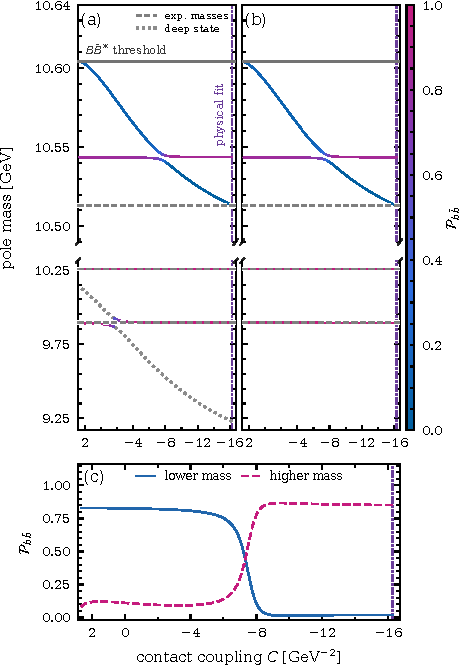
\includegraphics[width=\columnwidth]{levels_three_channel_projected.pdf}}
\caption{
Dependence of the four bound-state pole masses in the complete LO \BOchiEFT calculation for $N=4$, $\Lambda=4$~GeV, $m_b$ in Eq.~\eqref{mb}, and $V_0=371$~MeV on the contact coupling $C$.
Panels (a) and (b) show the results with the full OME potential and with the deep spurious state projected out, respectively; panel (c) shows ${\cal P}_{\bar{b}b}$ for the two near-threshold mass eigenstates of panel (b), illustrating the interchange of their compact-bottomonium content associated with the avoided level crossing.
The corresponding parameter values, together with $C=-16.27$~GeV$^{-2}$, marked by the vertical dot-dashed line close to the right edge of each plot, are given in Table~\ref{tab:schemes}.
The colour of each trajectory denotes its compact-bottomonium probability ${\cal P}_{\bar{b}b}$ defined in Eq.~\eqref{Pbb}. The dashed horizontal lines mark the three experimental $\chi_{b1}$ masses, while the solid horizontal line marks the $B\bar{B}^*$ threshold.
The grey dotted line in panel (a) corresponds to the regulator-dependent deep spurious pole removed by the projection method in panel (b).
}
\label{fig:levels}
\end{figure}





\bigskip


\acknowledgments
We acknowledge useful discussions with Eric Braaten, Nora Brambilla, Roberto Bruschini, Francesco Knechtli, Juan Nieves, Ulf-G. Mei\ss ner, Andreas Nogga, Mike Peardon, Tommaso Scirpa and Antonio Vairo.
This work is supported in part by the National Key R\&D Program of China under Grant No. 2023YFA1606703; by the National Natural Science Foundation of China (NSFC) under Grants No. 12125507, No. 12361141819, and No. 12447101, by the Chinese Academy of Sciences (CAS) under Grant No.~YSBR-101, and by
Deutsche Forschungsgemeinschaft (DFG) under Grant No. 576422137
and under Germany's Excellence Strategy -- EXC 3107 -- Project-ID~533766364. In addition, C.H., and A.N. thank the CAS President's International Fellowship Initiative (PIFI) for partial support under Grant Nos. 2025PD0087 and 2024PVA0004\_Y1, respectively.
Various AI agents were used for language polishing, cross-checking, code generation, and literature verifications, under the \texttt{nullius} harness framework~\cite{nullius}. The authors take full responsibility for the work.

\bibliography{refs}

\begin{appendix}
\section*{End Matter}
\noindent{\it OME potentials.---}Here we provide explicit expressions for the OME potentials (with $\phi$ denoting $\pi$ or $\eta$) in the $B^{(*)}\bar{B}^*$ system:
\begin{align}
&\VOME_{B\bar{B}^*\to B\bar{B}^*}(\vep',\vep;m_\phi)\label{VBBstBBst}\\
&=-\frac{g_b^2}{4F_\pi^2}(\veep\cdot \veq)(\veepst\cdot \veq) \left[D_{1}(\vep',\vep;m_\phi)+D_{2}(\vep',\vep;m_\phi)\right],\notag
\\[3mm]
&\VOME_{B\bar{B}^*\to B^*\bar{B}^*}(\vep',\vep;m_\phi)\label{VBBstBstBst}\\
&=\frac{g_b^2}{4F_\pi^2}\Big[({\veA_1}\cdot \veq)({\veep_2}^{\prime *}\cdot \veq)+({\veA_2}\cdot \veq)({\veep_1}^{\prime *}\cdot \veq)\Big] \notag\\
&\hspace*{0.3\columnwidth}\times\left[D_{3}(\vep',\vep;m_\phi)+D_{2}(\vep',\vep;m_\phi)\right],\notag
\\[3mm]
&\VOME_{B^*\bar{B}^*\to B\bar{B}^*}(\vep',\vep;m_\phi)\label{VBstBstBBst}\\
&=\frac{g_b^2}{4F_\pi^2}\Big[({\veA_1}\cdot \veq)({\veep_2}\cdot \veq)+({\veA_2}\cdot \veq)({\veep_1}\cdot \veq)\Big] \notag\\
&\hspace*{0.3\columnwidth}\times\left[D_{4}(\vep',\vep;m_\phi)+D_{2}(\vep',\vep;m_\phi)\right],
\notag\\[3mm]
&\VOME_{B^*\bar{B}^*\to B^*\bar{B}^*}(\vep',\vep;m_\phi)\label{VBstBstBstBst}\\
&\hspace*{0.15\columnwidth}=-\frac{g_b^2}{2F_\pi^2}(\veA_1\cdot \veq)(\veA_2\cdot \veq) \left[ 2D_{2}(\vep',\vep;m_\phi)\right], \notag
\end{align}
with the TOPT propagators of the form
\be
D_\beta(\vep',\vep;\mG)=\frac1{2\EG(q)\,[\EG (q)+\mu_\beta]},
\label{eq:Dbeta}
\ee
where $\beta=1,..,4$ labels the 3-body states in Eq.~\eqref{BBphichannels} in the main text, $\veq=\vep-\vep'$, and $\EG(q)=\sqrt{q^2+\mG^2}$. The nonrelativistically expanded $\mu_\beta$ functions are
\begin{align}
\mu_1&= m_B-m_{B^*}+\frac{p^2+p^{\prime2}}{2m_B}-E-i\epsilon, \notag \\
\mu_2&= m_{B^*}-m_B+\frac{p^2+p^{\prime2}}{2m_{B^*}}-E-i\epsilon, \notag\\
\mu_3&=\frac{p^2}{2m_{B}}+
\frac{p^{\prime2}}{2m_{B^*}}-E-i\epsilon, \label{eq:alphaOME}
\\
\mu_4&=\frac{p^{\prime2}}{2m_{B}}+
\frac{p^2}{2m_{B^*}}-E-i\epsilon. \notag
\end{align}
Isospin factors are omitted in Eqs.~\eqref{VBBstBBst}--\eqref{VBstBstBstBst}; for the isoscalar channel, these are 3 and 1/3 for $\pi$- and $\eta$-exchange, respectively.
In Eqs.~\eqref{VBBstBstBst}--\eqref{VBstBstBstBst}, subscripts $1$ and $2$ denote the incoming $B^*$ and $\bar{B}^*$ mesons: $\veep_1$ and $\veep_2$ ($\veep_1^{\prime *}$ and $\veep_2^{\prime *}$) are their incoming (outgoing) polarisations, and $\veA_a=\frac{i}{\sqrt2}(\veep_a\times\veep_a^{\prime *})$ for $a=1,2$. 
The $S$-wave projection of the OME potentials in Eqs.~\eqref{VBBstBBst}-\eqref{VBstBstBstBst} can be performed employing projectors technique as detailed in Ref.~\cite{Zhang:2026iyr}.

\end{appendix}

\end{document}

